\section{Messwerte und Auswertung}

\subsection{Sinusgitter} %fertig

Der Laser wird anhand des 2. Spiegels zentriert, dann werden das Sinusgitter und der Schirm eingebaut. Die Distanz zwischen den beiden Maxima 1. Ordnung ergibt sich aus der $x$- und der $y$-Verschiebung auf dem Schirm. Wir haben folgende Werte gemessen:
\begin{itemize}
\item $D_x = (9.9 \pm 0,1) cm$ (Distanz in $x$-Richtung)
\item $D_y = (1.1 \pm 0.1) cm$ (Distanz in $y$-Richtung)
\item $L = (5.9 \pm 0.3) cm$ (Distanz zwischen dem Gitter und dem Schirm)
\end{itemize}

Aus $D_x$ und $D_y$ ergibt sich die Distanz $D=\sqrt{D_x^2 + D_y^2} = 9.96$ mit dem Fehler
$$\sigma_D = \sqrt{\left(\frac{\partial D}{\partial D_x}\right)^2\sigma_{D_x}^2 + \left(\frac{\partial D}{\partial D_y}\right)^2\sigma_{D_y}^2} = \sqrt 2 \left(\frac{\partial D}{\partial D_x}\right)\sigma_{D_x} = \sqrt 2 \frac{D_x}{\sqrt{D_x^2 + D_y^2}}\sigma_{D_x} = \sqrt 2 \frac{D_x}{D}\sigma_{D_x} = 0,14$$

Somit: $$\boxed{D = (9.96 \pm 0.14) cm}$$

Es folgt der Winkel $\alpha$ aus $\tan(\alpha) = \frac{D}{2L} \Leftrightarrow\alpha = \arctan\left(\frac{D}{2L}\right) = 40.17^\circ$ mit dem Fehler

$$\sigma(\alpha) = \sqrt{\left(\frac{\partial \alpha}{\partial D}\right)^2\sigma_{D}^2 + \left(\frac{\partial \alpha}{\partial L}\right)^2\sigma_{L}^2} = \sqrt{\frac{L\sigma_D^2 + D\sigma_L^2}{2L(1+D^2/4L^2)}} = 0.22^\circ$$

Es folgt: $$\boxed{\alpha = (40.17 \pm 0.22)^\circ = (0.701 \pm 0.004) rad} $$

Die Gitterkonstante $K$ l\"asst sich somit berechnen: $$ K\sin(\alpha) = n\lambda \Leftrightarrow K = \frac{n\lambda}{\sin(\alpha)} = 9810.13 \ \mathring A \ \text{mit \ } n=1$$

$K$ besitzt den Fehler (unter Vernachl\"assigung des Fehlers auf $\lambda$): $$\sigma_K = \sqrt{\left(\frac{\partial K}{\partial \alpha}\right)^2\sigma_\alpha^2} = \frac{\lambda\cos(\alpha)\sigma_\alpha}{\sin^2(\alpha)} = 44.62 \ \mathring A$$

Somit folgt: $$\boxed{K=(9810 \pm 44) \ \mathring A = (981.0 \pm 4.4) \ nm}$$

Als Vergleich: Auf dem Gitter ist die Zahl der Linien pro Millimeter angegeben: \\ $g_{theo}=1016 L/mm$. Es folgt der Wert f\"ur die Gitterkonstante: $K_{theo} = 1/g_{theo} = 9842.52 \ \mathring A$, welcher sehr dicht an unserem ermittelten Wert liegt und innerhalb der ersten Standardabweichung.

\subsection{Bestimmung der Gitterkonstanten}

Wir haben den Strahlengang wie in 3.2.2 beschrieben justiert um eine m\"oglichst hohe Genauigkeit bei unserer Messung zu erhalten.

\subsubsection{Eichung anhand des Gitters R}

Sei $\Delta t$ die zeitliche Distanz zwischen 2 Nebenmaxima der Intensit\"atsverteilung. Die Distanz zwischen dem Hauptmaximum und einem Nebenmaximum ist somit $\Delta t/2$ und ist proportional zu $\sin(\alpha)$. Es gilt: $$\sin(\alpha) = \frac{n\lambda}{K} = \gamma \frac{\Delta t}{2}$$
Wir bestimmen die Proportionalit\"atskonstante $\gamma$ durch lineare Regression, indem wir $\Delta t/2$ gegen $n$ auftragen und den Steigungsfaktor $b$ ermitteln. Der Achsenabschnitt $a$ sollte idealerweise Null sein.

\begin{center}
\begin{tabular}{lllll}
\toprule
Peak & t in $\mu s$ & st in $\mu s$ & $\Delta t$ in $\mu s$ & $s\Delta t$ in $\mu s$ \\
\midrule
0. Ordnung \\
 & 501,0635 & 3,36E-002\\
\midrule
1. Ordnung\\
links & 404,7489 & 3,71E-002 & 192,4441 & 7,29084668847E-002\\
rechts & 597,193 & 3,59E-002\\
\midrule
2. Ordnung\\ 
links & 309,3735 & 2,07E-001 & 383,268 & 3,90324905236E-001\\
rechts & 692,6415 & 1,83E-001\\
\midrule
3. Ordnung\\ 
links & 214,3283 & 5,28E-001 & 573,2411 & 1,21769040489\\
rechts & 787,5694 & 6,89E-001\\
\bottomrule
\end{tabular}
\end{center}

Die Parameter der linearen Regression:
$$ b               = (9.53491e-05      \pm 9.823e-08) s    (0.103\%) $$
$$ a               = (8.74055e-07      \pm 1.043e-07) s    (11.94\%) $$

Der Achsenabschnitt $a$ ist also tatsächlich um einige zwei Größenordnungen kleiner als die Steigung $b$ und wird daher vernachlässigt. Somit erhalten wir den Zusammenhang

$$\frac{\Delta t}{2} = \frac{\lambda}{K\gamma}n = b\cdot n$$

den wir umstellen können nach $\gamma$, dem Proportionalitätsfaktor zwischen Zeit $t$ und Sinus des Winkels $\sin \alpha$ 

$$ \gamma = \frac{\lambda}{Kb} = (53.093317084272421 \pm 0.0546974909799) s^{-1} $$
%$$s\gamma = \frac{\lambda}{Kb^2} \cdot sb $$


\subsubsection{Bestimmung der Gitterkonstanten f\"ur die 5 Gitter}

Mit diesem Faktor können wir nun die Gitterkonstanten der anderen fünf Gitter aus dem Abstand der Maxima der ersten Ordnung bestimmen:
$$ g = \frac{\beta}{\lambda}\cdot \frac{\Delta t}{2} \text{ bzw. } k = \frac{2 \lambda }{\beta \Delta t} $$
\begin{center}
\begin{tabular}{lllll}
\toprule 
Gitter & $\Delta t /2$ in $\mu s$ & $s\Delta t /2$ in $\mu s$ & $k$ in $\mu m$ & $sk$ in $\mu m$\\
\midrule
G1 & 89.742 & 0.568 & 132.81 & 0.85\\
G3 & 112.111 & 0.205 & 106.31 & 0.22\\
G4 & 112.411 & 0.107 & 106.03 & 0.14\\
08540 & 113.490 & 0.677 & 105.02 & 0.64\\
08534 & 91.0123 & 0.139 & 130.96 & 0.24\\
\bottomrule
\end{tabular} 
\end{center}

F\"ur die beiden PHYWE-Gitter kennen wir den theoretischen Wert, n\"amlich: 
\begin{itemize}
\item PHYWE-08534: $g_{theo} = 8 L/mm\ \Rightarrow \ K_{theo} = 125 \ \mu m$
\item PHYWE-08540: $g_{theo} = 10 L/mm\ \Rightarrow \ K_{theo} = 100 \ \mu m$
%Vergleich mit dem exp. ermittelten Wert
Unsere Ergebnisse weichen relativ stark von den theoretischen Werten ab, wir vermuten das die Justierung mit Gitter ``R'' fehlerhaft ist. Ursache könnten Deformationen des Gitters ``R'' bedingt durch sein Alter und den häufigen Gebrauch sein. Falls nötig können wir die Eichung für die korrigierte Version nochmals mit einem der PHYWE-Gitter vornehmen.
\end{itemize} 

\subsection{Berechnung der Aperturfunktion f\"ur Gitter 1}

Wir nähern die Aperturfunktion mittels den Intensit\"aten der gemessenen Verteilung als Fourierreihe:
$$g(x) = \frac{\sqrt{I_0}}{2} + \sum_{n=1}^N \sqrt{I_n}\cos\left(\frac{2\pi n}{K}x \right)$$
F\"ur die $I_n$ haben wir folgende Werte ermittelt:

%Resultate I_0
\begin{tabular}{lll}
 \toprule
Ordnung & Amplitude & Fehler \\
\midrule
0. Ordnung & 5.5184706157133 & 0.0205159936960068 \\
1. Ordnung l & 0.221293372204415 & 0.00303468123804445 \\
1. Ordnung r & 0.154596997473865 & 0.00250997613519101 \\
2. Ordnung l & 0.147836581064078 & 0.00309767922452523 \\
2. Ordnung r & 0.135446035218821 & 0.00287225704831411 \\
3. Ordnung l & 0.0869833409521151 & 0.00328617199395248 \\
3. Ordnung r & 0.0952050159181131 & 0.00267868139085647 \\
\bottomrule
\end{tabular}


\begin{figure}[!h]
 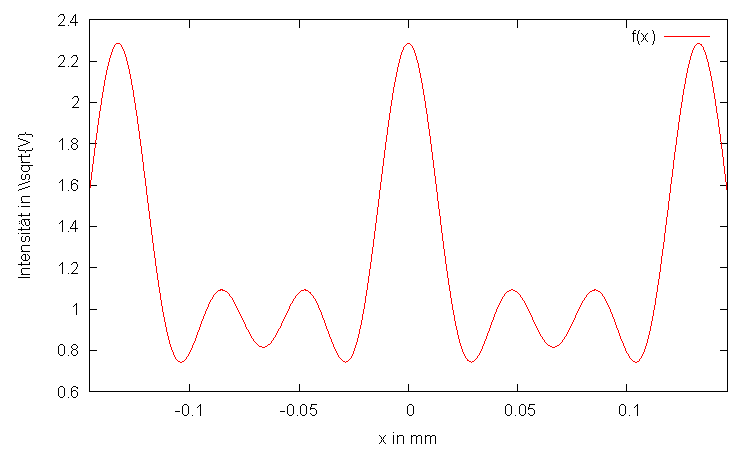
\includegraphics{Bilder/appertur.pdf}
\caption{Apperturfunktion mit $K = 130.96 \mu m $}
\end{figure}


\subsection{Bestimmung des Verh\"altnisses zwischen Spaltbreite und Spaltabstand}

Den maximalen y-Wert erhalten wir für $g\left( 0 \right) = \sqrt{I0}/2+\sqrt{I1}+\sqrt{I2}+\sqrt{I3} = y_{max} = 2.28627 $. Den minimalen y-Wert erhalten wir durch ablesen $ y_{min} = 0.743486 $. Die Halbwertsbreite $b$ mit $ g\left( - b/2 \right) = g \left( b/2 \right) = 1.51488 $ ergibt sich als $ b = 0.027334 $. Somit erhalten wir für das Verhältnis von Spaltbreite zu -höhe
$$ v = \frac{b}{K-b} = 0.26378 $$ %TODO Fehler? 

\subsection{Aufl\"osungsverm\"ogen der Gitter}

Das Aufl\"osungverm\"ogen $a$ ergibt sich bei normalen Gittern durch $a=N\cdot m$, wobei N die Zahl der durchleuchteten Maxima ist, und m die Zahl der sichtbaren Maxima. N bestimmen wir, indem wir die Laserbreite $b_L$ messen und durch die Gitterkonstante $K$ teilen.\\
Die Laserbreite haben wir mit dem Schirm gemessen und haben $b_L = (3.0 \pm 0.5) mm$ erhalten.\\
Es gilt also: $$N = \frac{b_L}{K}$$
mit dem Fehler: $$\sigma_N = \sqrt{\frac{\sigma_{b_L}^2K^2 + \sigma_K^2b_L^2}{K^4}}$$
Der Fehler auf $a$ ist: $$\sigma_a = \frac{\partial a}{\partial N}\sigma_N = m\cdot \sigma_N$$

Somit folgt f\"ur die Gitter:

\begin{itemize}
\item Gitter 1: $ a = 67.76575165317837 \pm 11.302658636724754 $
\item Gitter 3: $ a = 56.437974555788117 \pm 9.4070743547623081 $
\item Gitter 4: $ a = 28.294658556680321 \pm 4.7159427734459909 $
\item PHYWE 08540: $ a = 28.566288540708861 \pm 4.764184123944938 $
\item PHYWE 08534: $ a = 45.816820585847005 \pm 7.6366043023007304 $
\end{itemize}


\subsection{Raman-Nath-Theorie}

\begin{verbatim}
 werte[0.0][0] = 7.81411; s[0][0] = 0.05;
  werte[0.0][1] = 0.534180; s[0][1] = 0.05;
  werte[0.0][2] = 0.165152; s[0][2] = 0.05;
  
  werte[1.01][0] = 7.58345; s[1.01][0] = 0.05;
  werte[1.01][1] = 0.595606; s[1.01][1] = 0.05;

  werte[2.0][0] = 7.18386; s[2][0] = 0.05;
  werte[2.0][1] = 0.911210; s[2][1] = 0.05;
  
  werte[3.0][0] = 6.65979; s[3.0][0] = 0.05;
  werte[3.0][1] = (0.988260 + 1.06716) /2; s[3.0][0] = 0.03 / sqrt(2.);
  
  werte[3.99][0] = 5.90614; s[3.99][0] = 0.04;
  werte[3.99][1] = (1.32051 + 1.37895) / 2; s[3.99][1] = 0.01 / sqrt(2.);
  werte[3.99][2] = 0.1459; s[3.99][2] = 0.04;
  
  werte[4.99][0] = 5.10557; s[4.99][0] = 0.05;
  werte[4.99][1] = (1.67044 + 1.71344) / 2; s[4.99][1] = 0.05 / sqrt(2.);
  werte[4.99][2] = 0.232797; s[4.99][2] = 0.1;
  
  werte[5.66][0] = 4.46693; s[5.66][0] = 0.04;
  werte[5.66][1] = ( 1.98781 + 1.98498)/ 2; s[5.66][1] = 0.04 / sqrt(2);
  werte[5.66][2] = 0.307564; s[5.66][2] = 0.04;
  
  werte[6.34][0] = 3.76185; s[6.34][0] = 0.02;
  werte[6.34][1] = (2.18152 + 2.20363) /2; s[6.34][1] = 0.03 / sqrt(2);
  werte[6.34][2] = (0.366363 + 0.345704) / 2; s[6.34][2] = 0.03 / sqrt(2);
  
  werte[7.00][0] = 3.16188; s[7][0] = 0.02;
  werte[7.00][1] = (2.40147 + 2.40510) / 2; s[7][1] = 0.03 /sqrt(2);
  werte[7.00][2] = (0.482917 + 0.445933) / 2; s[7][2] = 0.03 / sqrt(2);
  
  werte[7.68][0] = 2.58162; s[7.68][0] = 0.03;
  werte[7.68][1] = (2.56090+2.54017)/2; s[7.68][1] = 0.03 / sqrt(2);
  werte[7.68][2] = (0.604586+0.558788) / 2; s[7.68][2] = 0.03 / sqrt(2);
  
  werte[8.33][0] = 1.64141; s[8.33][0] = 0.03;
  werte[8.33][1] = (2.76328 + 2.72248)/2; s[8.33][1] = 0.02 / sqrt(2);
  werte[8.33][2] = (0.819292 + 0.782161)/2; s[8.33][2] = 0.03 / sqrt(2);
  werte[8.33][3] = (0.162417 + 0.121085)/2; s[8.33][3] = 0.03 / sqrt(2);
  
  werte[8.99][0] = 1.20705; s[8.99][0] = 0.03;
  werte[8.99][1] = (2.74320 + 2.74059 )/2; s[8.99][1] = 0.03 / sqrt(2);
  werte[8.99][2] = (0.985601 + 0.887822 ) / 2; s[8.99][2] = 0.03 / sqrt(2);
  werte[8.99][3] = (0.177135 + 0.139159 ) / 2; s[8.99][3] = 0.03 / sqrt(2);
  
  werte[9.69][0] = 0.970063; s[9.69][0] = 0.04;
  werte[9.69][1] = (2.65724 + 2.66896)/2; s[9.69][1] = 0.03 / sqrt(2);
  werte[9.69][2] = (1.10564 +  1.04613) / 2; s[9.69][2] = 0.04 / sqrt(2);
  werte[9.69][3] = (0.231922 +  0.189630) / 2; s[9.69][3] = 0.04 / sqrt(2);
\end{verbatim}
 

Durch Ablesen haben wir die Intensität der Maxima bestimmt. Diese haben wir dann mit der Intensität des Hauptmaxima bei ausgeschalteter Spannung $I_0 = $ normiert. Der Fehler ergibt sich dann durch $sI = \frac{I}{I0} * \sqrt{\left(\frac{sI}{I}\right)^2 + \left(\frac{sI_0}{I_0}\right)^2}$.

Die in der Anleitung empfohlene Verwendung des 1. Minimums bei der Nullten Ordnung zur Bestimmung des Skalierungsfaktors $ a $ konnten wir leider nicht befolgen, da dieses Minimum bei nicht durch unsere Messwerte abgedeckt wurde. Daher haben wir den Faktor alternativ durch Fitten der Funktion $J_0(a_0*x)$ an die 0. Ordnung bzw. $J_1(a_1*x)$ an die 1. Ordnung ermittelt. Wir erhalten dabei $a_0 = 1.8453e-01 \pm 3.7e-04$ sowie $a_1 = 2.3449e-01 \pm 7.0e-04 $ und verwenden für die restlichen beiden Ordnungen den Mittelwert $a = 2.09508e-01$. 

\begin{figure}[H]
 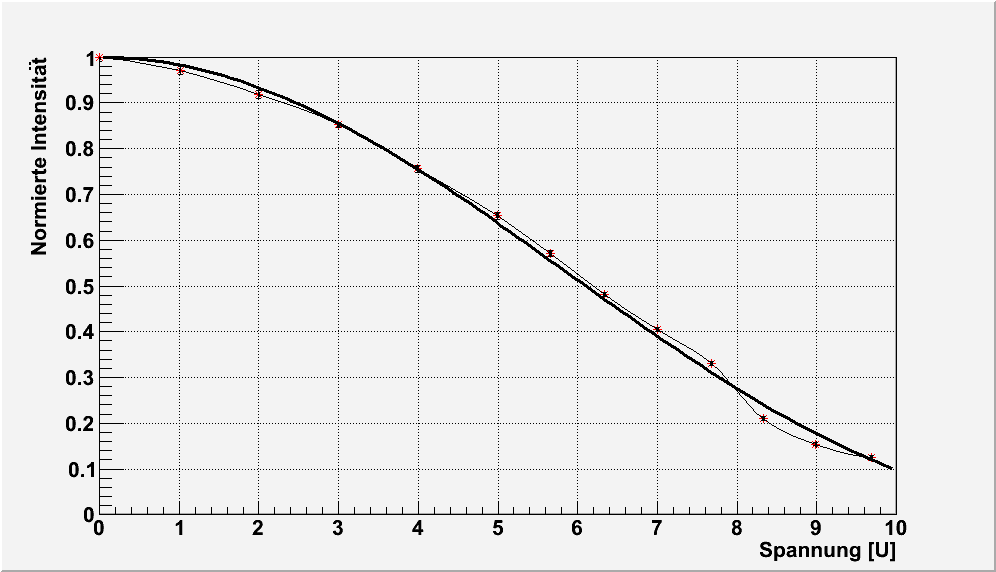
\includegraphics[width=0.9\textwidth]{Bilder/raman/raman-fit_0.png}
 \caption{Vergleich 0. Beugungsordnung mit $J_0^2$}
\end{figure}
Die Intensitäten der nullten Ordnung passen also gut zum Verlauf, der aus der Raman-Nath-Theorie erwartet wurde.
\begin{figure}[H]
 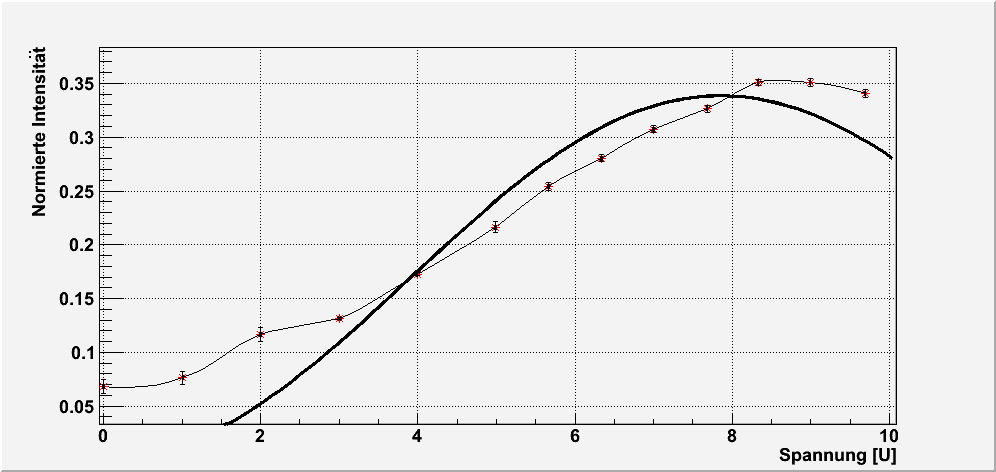
\includegraphics[width=0.9\textwidth]{Bilder/raman/raman-fit_1.png}
 \caption{Vergleich 1. Beugungsordnung mit $J_1^2$}
\end{figure}
Die Intensitäten der ersten Ordnung passen ebenfalls zur Raman-Nath Theorie, allerdings nicht besonders gut.
\begin{figure}[H]
 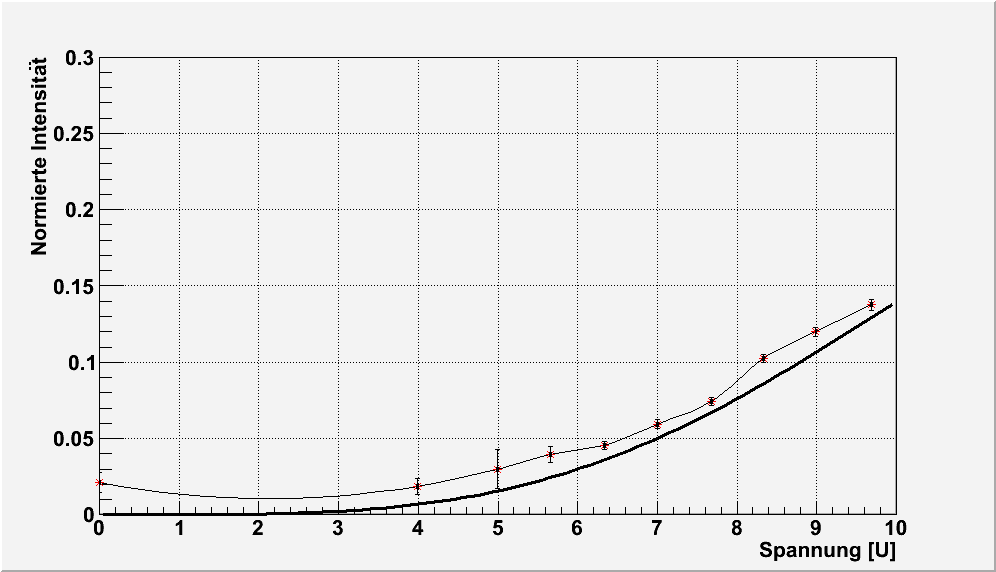
\includegraphics[width=0.9\textwidth]{Bilder/raman/raman-fit_2.png}
 \caption{Vergleich 2. Beugungsordnung mit $J_2^2$}
\end{figure}
Für die zweite Ordnung ist die Übereinstimmung mit der Theorie wieder etwas besser, der Wert bei $U=0V$ scheint allerdings falsch zu sein.
\begin{figure}[H]
 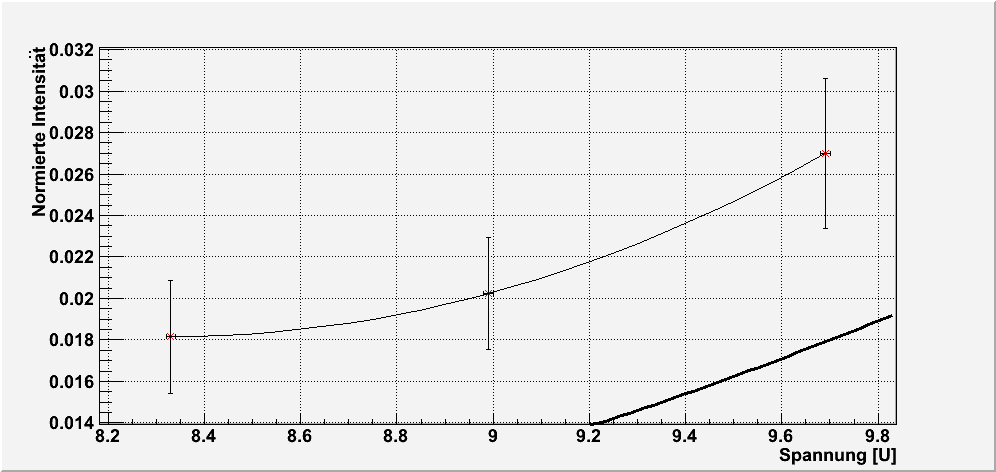
\includegraphics[width=0.9\textwidth]{Bilder/raman/raman-fit_3.png}
 \caption{Vergleich 3. Beugungsordnung mit $J_3^2$}
\end{figure}
Da wir die dritte Beugungsordnung nur bei wenigen Spannungen beobachten konnten, eignet sie sich nicht für eine Aussage zur Gültigkiet der Raman-Nath-Theorie.

\subsubsection{Ultraschallwellenlänge}

Für die Ermittlung der Schallwellenlänge haben wir die Messung bei $ U = 9.69 V$ und $f = 2109.195 kHz $ verwendet. Dazu haben wir die Zeit $t$ der Maxima gegen ihre Ordnung aufgetragen. Aus der Steigung $a$ einer Ausgleichsgeraden erhalten wir über den Zusammenhang 
$$ \sin \alpha = \frac{m \lambda}{\lambda^{*}} = \beta \frac{\Delta t}{2} $$
 die Schallwellenlänge $ \lambda^* $


\begin{table}[H]
\begin{center}
\caption{Steigung und Achsenabschnitt der Ausgleichsgeraden}
\begin{tabular}{llll}
\toprule
Parameter & Wert & Fehler & \\
\midrule
a & 2.07162e-05   &  $ \pm 9.1e-08$  &    $(0.4392\%)$\\
b & 9.85261e-05 & $ \pm 1.966e-07$ &   $(0.1995\%)$ \\
\bottomrule
\end{tabular}
\end{center}
\end{table}


Aus $ \beta \frac{\Delta t}{2} = a m + b = \frac{\lambda}{\lambda^*} m + b $ folgt 
$$\boxed{ \lambda^* = \frac{\lambda}{\beta a} = 575.329 \mu m}$$

Der Achsenabschnitt enthält nur den Offset und ist nicht weiter von Bedeutung. 















